%\documentclass[11pt]{report}
\documentclass[10.5pt, a4paper]{report}
\usepackage{sectsty}
\usepackage{ltablex}
\usepackage[style=apa]{biblatex}
\addbibresource{references.bib}
\usepackage{hyperref}
% Colors 
%\usepackage{color}
\usepackage[dvipsnames, table]{xcolor}
\definecolor{my_pine_green}{cmyk}{100, 0, 18, 48}
\definecolor{my_navy}{cmyk}{0.99, 0.5, 0.0, 0.40}
\definecolor{my_green}{cmyk}{0.96, 0.0, 0.64, 0.40}
\definecolor{cadet}{rgb}{0.33, 0.41, 0.47}
\chapternumberfont{\LARGE} 
\chaptertitlefont{\Huge}
\usepackage[
	top    = 2.20cm,
	bottom = 2.20cm,
	left   = 2.82cm,
	right  = 2.20cm,
	includeheadfoot]{geometry} % Use similar margins to the Word Template

% \usepackage[left=1.5in, right=1in, top=1in, bottom=1in, includefoot, headheight=13.6pt]{geometry}
% \usepackage{pslatex}	% Use PostScript Fonts
\usepackage[utf8]{inputenc}
\usepackage{graphicx}
\graphicspath{ {images/} }
\usepackage{amsmath}
\usepackage{amssymb}
\usepackage{caption}
\usepackage{subcaption}
\usepackage{float}
\usepackage{fancyhdr}
\usepackage[T1]{fontenc}
\renewcommand{\baselinestretch}{1.4}
\usepackage{multirow}
\usepackage{makecell}
\usepackage{amsmath}
\usepackage{booktabs}
\usepackage{siunitx}
\newcommand{\foo}{\foo} 
\DeclareMathOperator*{\argmax}{argmax} % thin space, limits underneath in displays
\newcolumntype{P}[1]{>{\centering\arraybackslash}p{#1}}

\hypersetup{
    colorlinks=true,
    linkcolor=my_navy,
    filecolor=magenta,      
    urlcolor=my_navy,
    citecolor=my_navy,
}

\usepackage[ruled]{algorithm2e}

\newcommand{\blankpage}{
    \newpage
    \thispagestyle{empty}
    \mbox{}
    \newpage
}

% Page Header
\pagestyle{fancy}

\renewcommand{\chaptermark}[1]{\markboth{#1}{}}
\fancyhf{} % clear the headers
\fancyhead[R]{%
   % We want italics
   \itshape
   % The chapter number only if it's greater than 0
   \ifnum\value{chapter}>0 \chaptername\ \thechapter. \fi
   % The chapter title
   \leftmark}
\fancyfoot[C]{\thepage}

\fancypagestyle{plain}{
  \renewcommand{\headrulewidth}{0pt}
  \fancyhf{}
  \fancyfoot[C]{\thepage}
}

\setlength{\headheight}{14.5pt}


\usepackage[ruled]{algorithm2e}

\newcommand{\blankpage}{
    \newpage
    \thispagestyle{empty}
    \mbox{}
    \newpage
}

\usepackage{makecell}

\title{Master thesis title}
\author{Sohyung Kim}
\date{\today}

\usepackage[intoc, english]{nomencl}
\makenomenclature

\begin{document}

% Title page
\begin{titlepage}
    \begin{center}
        \vspace{0.5cm}
        
        
\includegraphics[width=\textwidth]{images/banner.png}
        
        \vspace{1cm}
        
        \textbf{Department of Artificial Intelligence}\\
        \textsc{Master's thesis}
        
        \vspace{0.5cm}
        
        \LARGE
        \noindent\rule{13cm}{0.8pt}
        \textbf{Using Confidential Data for Domain Adaptation of Neural Machine Translation}
        \noindent\rule{13cm}{0.8pt}
        
        \vspace{2cm}
        
        \normalsize
        \textbf{Author}\\
        Sohyung Kim\\
        S3475743\\
        \vspace{0.5cm}
        \textbf{First Supervisor}\\
        University of Groningen\\
        \vspace{0.5cm}
        \textbf{Second Supervisor}\\
        
        
        \vfill
        \today
    \end{center}
\end{titlepage}
\blankpage

% Nomenclature 
% \nomenclature{$\theta$}{Master policy}
% \nomenclature{$\phi$}{Sub policy}
% \nomenclature{$I_{\phi}$}{Number of sub-policy updates in each cycle}
% \nomenclature{$I_{\theta}$}{Number of master policy updates in each cycle}
% \nomenclature{$P_T$}{All the different tasks that are available in the environment}
% \nomenclature{$\rho$}{Success threshold}
% \nomenclature{$N$}{Number of timesteps worth of experience}
% \nomenclature{$C$}{Number of training cycles/episodes}
% \nomenclature{$R$}{Remind frequency}
\nomenclature{AI}{Artificial Intelligence}
\nomenclature{MT}{Machine Translation}
\nomenclature{SMT}{Statistical Machine Translation}
\nomenclature{NMT}{Neural Machine Translation}
\nomenclature{ML}{Machine Learning}
\nomenclature{NLP}{Natural Language Processing}
\nomenclature{OOV}{Out-Of-Vocabulary}
\nomenclature{LSTM}{Long Short-Term Memory}


% Chapters
\pagenumbering{roman}
\chapter*{Abstract}
\addcontentsline{toc}{chapter}{Abstract}%
Domain adaptation has led to remarkable achievements in Neural Machine Translation (NMT). Therefore, the availability of in-domain data remains essential to ensure the quality of NMT, especially in technical domains. However, obtaining such data is often challenging, and in many real-world scenarios this is further aggravated by data confidentiality or copyright concerns. 

We study the problem of domain adaptation in NMT when domain-specific data cannot be shared due to confidentiality issues. We propose to fragment data into phrase pairs and use a shuffled and random sample to fine-tune a generic NMT model instead of using the full sentences. Despite the loss of long segments, we find that NMT quality can considerably benefit from this adaptation and that further gains can be obtained with a simple tagging technique.

% %Domain adaptation has led to remarkable achievement in Machine Translation.
% We study the problem of domain adaptation in Neural Machine Translation (NMT) when domain-specific data cannot be shared due to confidentiality or copyright issues.
% %However, in order to expect good performance in such domain adaptation, the provision of sufficient in-domain data should be required. Due to confidentiality concerns, highly sensitive data is not always shareable, and the data lost the opportunity to be shared can result in poor MT quality. 
% We propose to fragment data into phrase pairs and use a random sample to fine-tune a generic NMT model instead of the full sentences. 
% %We study whether this fragmented data could be used for domain adaptation of NMT. We propose phrases as a fragmented parallel corpus for domain adaptation. 
% Despite the loss of long segments, %because of phrase extraction, 
% we find that NMT quality can considerably benefit from this adaptation, and that further gains can be obtained with a simple tagging technique. 
\medskip


\textbf{\emph{Keywords}} --- Confidential Data/ Domain Adaptation/ Neural Machine Translation / Phrase Pairs / Fine-tuning/ Transformer
\chapter*{Acknowledgements}
\addcontentsline{toc}{chapter}{Acknowledgements}%
\input{chapters/acknowledgements}


\printnomenclature

\tableofcontents

\clearpage
\pagenumbering{arabic}

\chapter{Introduction}\label{chapter:introduction}
\newcommand{\SH}[1]{{\small\textcolor{blue}{[ #1]}}}


%The emergence of substantial amounts of digitized text gives rise to train machine learning models for various downstream applications.
% With the rapid growth of international markets, the need for translation has also been increasing.
%Furthermore, since the quality of MT has been improving as a 'good enough' translation that can replace human translator for regular and no need precise translation task, many companies also provide MT services. 
%and in order to have better communication, accurate translation is important??.. Therefore machine translation (MT) is an important research area, as a result. \\ typically modeling entire sentences in a single integrated model.
%%%% Introduce MT and NMT
With the growth of the international market and the freedom to share information through the Internet, the need for translation is increasing exponentially. It is getting difficult to meet this explosive demand for translation by only human translators due to cost and time constraints. Accordingly, an approach to Machine translation (MT), automatically translating one language into another language,
has continuously received significant attention in Artificial Intelligence (AI). 
%with or without human assistance, 

Hence many generations of MT models have evolved since the early 1950s, when the first practical MT models were suggested~\parencite{hutchins2007machine}.
%a relatively long period of time. 
%One of the dominant frameworks of the previous generation for MT research was Statistic Machine Translation (SMT).
For a while, Statistic Machine Translation (SMT) was the dominant framework for MT research and industry. However, more recently, Neural Machine Translation (NMT)~\parencite{kalchbrenner-blunsom-2013-recurrent, bahdanau2014neural}, which uses neural network models to solve MT task, has replaced SMT with significant progress.
One of the main reasons NMT outperforms other traditional MT models is that it is trained in end-to-end fashion. While SMT consists of subsequent components that are trained separately, NMT instead combines all of the components into one big trainable encoder-decoder structured model. This allows NMT to be able to have better exploitation of context than SMT.

%%%%% Limitation of availability of in-domain data the adequate supply of training data
%when have large volumes of language data. What still appears to be the main bottleneck is the lack of data in a particular target language or domain.
Although NMT yields state-of-art performance, it still shows several weaknesses. The most common problem is that NMT relies heavily on training data like other deep learning models because it has an architecture based on deep neural networks. This means that it is not only data-hungry but also very sensitive to the domain difference between training and test data. Many researches reported that NMT performs poorly for domain specific translation in the low resource scenarios~\parencite{zoph2016transfer, koehn-knowles-2017-six, ostling2017neural, sato-etal-2020-vocabulary}. However, in practice, extensive scale parallel data (several million sentences) is available only in limited language pairs and domains. To cope with this data scarcity, domain adaptation --- using knowledge of the source domain to improve the performance of the target domain --- is frequently used.
In particular, as a conventional domain adaptation technique for NMT, fine-tuning~\parencite{freitag2016fast, chu-etal-2017-empirical} is employed in the case where the large out-domain and relatively small in-domain parallel datasets are feasible.

%raise the issue - confidential data cannot be used for NMT improvement 
The availability of high quality in-domain data, therefore, remains essential to ensure the quality of NMT, especially in technical domains~\parencite{koehn-knowles-2017-six}. However, obtaining such data is still challenging. In many real-world scenarios, this is further aggravated by data confidentiality or copyright concerns. For example, in a scenario where a translation company based on a pipeline of NMT and human post-editing, the company wants to use its clients' data and translation for improving the NMT quality. In fact, when data content is highly sensitive, the owner of the data (the clients of the translation company) may simply deny providing its data and translation to the translation company it is hiring \parencite{cancedda-2012-private}. Missing the opportunity to use such sensitive in-domain data can lead to considerably worse MT quality, higher post-editing efforts and subsequently higher translation costs for the data owners themselves. In this context, we begin to question the feasibility of exploiting the parallel datasets that cannot be used for reasons of confidentiality to improve NMT quality. If a NMT system can take advantage of any part of high-quality in-domain data, the data owner and the translation company could benefit together from reduced post-editing cost. 
%We consider releasing such data in fragmented form as an alternate, to protect the confidentiality, even if it hurts the usefulness of the data.


%%%%% Enter: NLP for Privacy Angle 
Our main observation is that, in natural language processing (NLP), when the complete data cannot be shared in its original form, releasing \textit{fragmented} data can be considered as a compromise. The most well-known example of releasing fragmented data is \textit{Google N-gram} \parencite{michel2011quantitative}. N-gram tables consisting of sequences of \textit{n} words and their counts in a given corpus were routinely used to train count-based language models \parencite{kneser-ney, brants-etal-2007-large} before the advent of neural methods. However, fragmented data like N-grams is not optimal for training state-of-the-art NMT models that are based on deep neural networks
%Even though the fragmented dataset can keep confidentiality, however, it will trade-off data usefulness for training NMT models.
such as sequence-to-sequence LSTM \parencite{sutskever2014sequence} or Transformers \parencite{vaswani2017attention}. As mentioned above, one of the main strengths of these models is the ability of handling arbitrarily long contexts, which would be hindered by the use of fragmented data. 
%In addition, since parallel data is requisite for training NMT, fragmented data for NMT have to remain the alignments. 
In this thesis, we take a pragmatic approach and ask: If the data owner can \textit{only} release fragmented data due to confidentiality issues, can this still benefit downstream NMT quality in any way? As a solution, we propose \textit{phrase pairs} for a fragmented text format. Phrase pairs are one of the major components of phrase-based MT that keeps word alignments.

Motivated by the brittleness of NMT in out-of-domain settings \parencite{koehn-knowles-2017-six} and the increasing availability of large pre-trained models \parencite{ng-etal-2019-facebook}, in this thesis, we focus on the task of adapting a strong-performing general-domain pre-trained NMT system to various technical domains. As a viable solution to exploit confidential data, we fine-tune phrase pairs of in-domain data as parallel sentences. Furthermore, to maximise the utility of phrase pairs for fine-tuning a NMT model while preserving the confidentiality of data, we devise various methods for presenting phrases to models.
    
%In order to train such deep learning models, these the training needs the whole sentences and learn the context from them. However, phrases break down the sentences and while doing it it can lose some of the contextual information. Therefore, fragmented data is not useful way to share the textual data in NMT models. Here, the question can arise : If the data owner can release only phrases because of confidentiality, is there any way to use this to improve the NMT model? In this project, we will explore the possibility of using otherwise unavailable confidential data to improve NMT models. In our experiments we will be focusing on domain adaptation, therefore we consider ways to improve pre-trained neural models with phrases. 
%Rapid development of neural machine translation (NMT) has led to the improvement in MT. However, due to the nature of deep learning models, the quality and availability of abundant data is required for good performance. In the case of poor resource, NMT is either worse than or comparable to the statistical machine translation (SMT) models\parencite{zoph2016transfer}. In order for dealing with the data scarcity problem, many researches have been studied. Domain adaptation is an effective method and has fulfilled a key role in recent astonishing advances in Neural Machine Translation (NMT).
%When the complete data cannot be shared in its original form, as a compromise, releasing some statistics or fragmented data can be considered. The most well-known example of releasing fragmented data is Google N-gram \parencite{michel2011quantitative}. N-grams consist of sequences of \textit{n} words and counts in the given corpus and the idea behind it is how many words should be considered to predict the next word. 
%To specify the scenario for our study, we consider a case where a company provides an NLP service based on deep learning methods. This company may want to improve their models' performance by training or adapting to the clients' data. Due to confidentiality concerns, the clients only provide N-grams and counts of the original data as a compromise. In this case, if the N-gram can be used to improve the NLP model, both the clients and the company will benefit. Since the company can use this fragmented data to improve their solutions, the clients will receive better service. In this point of view, we want to study the possibility of sharing N-grams for improving utility while preserving privacy of data.
%Some studies have already discussed about it in the past for statistical models\cite{cancedda2012private}. However, we need a different approach in the context of deep learning based on NLP technologies. Currently, deep neural network, such as LSTM or transformer, has been used for solving the NLP tasks. In order to train these deep learning models, these models need the whole sentences and learn the context from them. However, N-grams break down the sentences and while doing it it can lose some of the contextual information. Therefore, N-gram is not useful way to share the textual data in these days. Here, the question can arise : If the data owner can release only N-grams because of confidentiality, is there any way to use this to improve the deep learning NLP model? 



\section{Research Questions}\label{section:research_questions}

This project aims to answer the following research question:

\begin{quote}

\textit{In the scenario where the original data is not shareable due to confidentiality issues and \textbf{only shuffled phrase pairs} can be released as a compromise, can this benefit downstream NMT quality in any way?}

\end{quote}
%The topic is training neural language models and/or NMT models on fragmented data (e.g. n-grams) in the scenario where the original data cannot be released in its original form for copyright or confidentiality reasons.

\noindent We will address the main research question by answering the following sub-questions:

\begin{enumerate}
    % Improvement ? 
    \item How much does the translation quality of out-of-domain models improve over the baseline models when fine-tuning on in-domain phrase pairs?

    % different maximum length - how different effect?
    \item %We can intuitively expect shorter phrases to lose more contextual information. Based on this, can we see that if use a shorter maximum phrase length, the quality of the translation is lowered?
    Does the use of shorter phrases (i.e. more fragmented data) lower translation quality?
    
    \item Can the phrase adapted NMT model's translation quality be improved by applying tagging techniques to present phrase pairs to the NMT model?
    
    % interesting differences between domains?
    \item When fine-tuning the NMT model on phrase pairs, are there any significant differences between different test domains?
    
    % Which method works best among all the combinations of our methods? and how is different in domains?
    %\item Can applying the tagging technique for presenting the phrases to NMT model improve the translation quality? 
    
\end{enumerate}

%\section{Contributions}
% The main contributions of this paper are the following:

% \begin{itemize}
%     \item We propose a novel idea that using phrase pairs 
% \end{itemize}

% Some of the work presented in the course of this thesis

\section{Thesis Outline} \label{section:thesis_outline}
This thesis is organised as follows.
%In this section, we briefly summarise the structure of the paper. 
Chapter~\ref{chapter:MT} provides some background on NMT and domain adaptation. In Chapter~\ref{chapter:methodology}, we propose our approach for answering the research questions with a motivated scenario. Chapter~\ref{chapter:experimental_setup} provides all details of our experiments. We evaluate the results of all experiments and represent analysis of the results in chapter~\ref{chapter:results}.
Finally, we answer the research questions and conclude our findings with possible future work in Chapter~\ref{chapter:conclusion}. 

Part of this thesis has been published as a workshop paper~\parencite{kim-etal-2021-using}.
\chapter{Background}\label{chapter:MT}
%There are some concepts that the reader should be familiarised with in order to fully understand the work described in the following chapters. These concepts are briefly explained in this chapter in order to contextualize and help the reader understand the rest of this writing.

\section{Neural Machine Translation}

Neural machine translation(NMT) has achieved

\section{Encoder-Decoder Architectures}

Limitations of Encoder-Decoder Networks

\section{Attention based encoder decoder Framework}
\subsection{Transformers}
The Transformer is a deep learning model proposed in the paper Attention is All You Need 
\section{Domain Adaptation for Neural Machine Translation}
\section{Regularization Techniques}
\parencite{arpit2017closer} suggested several regularization techniques to prevent overfitting. \\
\subsection{Early stopping}
\subsection{Dropout}
\subsection{Weight decay}

% \chapter{Related Work} \label{chapter:related_work}
% \input{chapters/related_work}
\chapter{Methodology} \label{chapter:methodology}
\section{Data}\label{section:datasets}

% Before selecting the out-domain dataset, we try to replicate the experiment of Fairseq WMT19 News translation task in German $\rightarrow$ English language direction. We evaluate the models on four domains including in-domain. 
\begin{table}[h] 
\centering
\begin{tabular}{cccc}
\hline
        & Documents  & Sentences & Tokens \\ \hline
EMEA    & 1939    &1108716    & \\ 
JRC    & 12035    & 2561711   & \\ 
GNOME    & 2280    &    & \\ \hline
\end{tabular}
\caption{Short description of datasets}
\label{Tab:Dataset}
\end{table}
We evaluate our experiments on German → English translation task , where the parallel corpora is publicly available from different domains: EMEA, GNOME and JRC-Aquis(JRC). These parallel corpora are from the OPUS project\parencite[]{tiedemann2012parallel}. EMEA(European Medicines Agency documents) is consisted of PDF documents from the European Medicines Agency. JRC-Acquis is a collection of legislative text of the European Union and currently comprises selected texts written between the 1950s and now.


\subsection{Data Preprocessing}

\subsubsection{Parallel Corpora Filters}

There are several common defects from the parallel corpora that can affect the quality of NMT models. Therefore, we filter out parallel corpora. We used the standalone XML format parallel corpora from OPUS.  

1. Extract the pure sentenced from standalone XML format target and source files. In order to extract it with the correct/ right alignments, we use OPUS tool which can help to extract the well aligned sentences from both languages files.

2. Remove duplicated sentences - which caused too high BLEU score. \\
3. clean up the short sentences :Also, too short sentences or empty sentence were cleaned out.($<$ 8 words). \\
4. alignment issues: some sentences in parallel corpus are missing. Thus they were removed.( which will causes problems with applying fast alignment) \\

6. Keep the information of documents of sentences. For example, we knows which documents were used for making for each datsets(train/valid/test). This is because it might be used for later to check up the confidentiality(need to think more about this..)

%The format of raw data is normally XML(Extensible Markup Language) 
%xml parser : The xml.etree.ElementTree module implements a simple and efficient API for parsing and creating XML data.
%The XML tree structure makes navigation, modification, and removal relatively simple programmatically. Python has a built in library, ElementTree, that has functions to read and manipulate XMLs (and other similarly structured files).
should mention about \cite{aulamo-etal-2020-opustools}


\subsection{Byte Pair Encodings}
Before training or finetuning NMT, creating sub-word vocabulary is important. This is because of the sub-word vocabulary can affect significantly to the performance of the NMT models. In this project, fastBPE is used.%need more explanation :D
Fairseq team used joint byte pair encodings (BPE) with 32K split operations for subword segmentation. 
Furthermore, for the WMT19 model, Fairseq team used their own \textit{fastBPE} to apply BPE on the datasets. 

\section{Phrase based Machine Translation}
\subsection{Fast Alignment}
\subsection{Moses Phrase Extraction}
\section{Evaluation Metrics}\label{section:evaluation_metrics
}
BLEU score / SacreBLEU 

\section{Fairseq WMT19 Neural Machine Translation model}

\chapter{Experimental Setup}\label{chapter:experimental_setup}
In the previous chapter, we introduced our motivating scenario and the main ideas for answering the research questions. 
Based on this, the current chapter describes the setup of the experiments that are carried out in this thesis. %The following sections provide details of the experiments. 
Section~\ref{section:baseline} explains the baseline model that we use for all our experiments as an out-domain pre-trained model. Then, Section~\ref{section:datasets} provides the details of in-domain datasets and preprocessing steps applied to the datasets. Section~\ref{section:phrase_extraction} explains the process of extracting phrase pairs from the in-domain datasets. Finally, Section~\ref{section:fine-tuning} covers the details of fine-tuning processes. In particular, we show the several methods for presenting phrase pairs to the NMT model during fine-tuning.


\section{Baseline Model}\label{section:baseline}

We use the Transformer-based NMT system \parencite{vaswani2017attention} pre-trained by Facebook for the WMT'19 news translation task \parencite{ng-etal-2019-facebook}. It is released as part of the \textsc{Fairseq} toolkit \parencite{ott-etal-2019-fairseq}\footnote{\url{https://github.com/pytorch/fairseq}}. This model basically follows a big Transformer architecture from \cite{vaswani2017attention}, except using the larger feed-forward network (FFN) sub-layers size (8192). It was trained on Paracrawl 27.7M sentences, and was fine-tuned on several previous years WMT news-test sets for an additional epoch. Fairseq team released an ensemble of these four models but for our study we only use 'model 1'. 
%To simulate a realistic production setup, we start from a strong NMT sys- tem pre-trained on large amounts (28M sentences) of publicly available data.

Based on our scenario, to simulate a realistic production setup, a baseline model that has high performance for out-domain translation is required. This model satisfies this requirement: It was ranked first in the WMT'19 news competition \parencite{barrault-etal-2019-findings} with a BLEU score of 40.8 on a German-English news task. 


\section{Data}\label{section:datasets}
%why we chose public data instead of confidential data
%In the scenario (Section~\ref{section:scenario}), the original data is highly sensitive since it contains core information that the data owner wants to protect. 
We simulate the scenario of confidential data by using publicly available datasets in several technical domains: medicine descriptions, software manual and EU legislation. We consider these domains because they generally contain sensitive information that an adversary may abuse for profit or other reasons. 

%Short description of datasets
We evaluate our approach on a German to English translation task. For different technical domains, we choose EMEA (medical), GNOME (software) and JRC-Acquis (legal)~\parencite{steinberger2006jrc}. EMEA is a parallel text of medical guidelines from European Medicines Agency. GNOME is a collection of the text from GNOME desktop environment and software platform. JRC is a collection of legislative text from the European Union. All the public corpora are from the OPUS project \parencite[]{tiedemann-2012-parallel}\footnote{\url{https://opus.nlpl.eu/}}.%Note that, for avoiding confusion, we refer to JRC-Acquis as JRC in this paper. 

\subsection{Preprocessing}

For a realistic simulation of a professional translation scenario, we split the datasets by documents. This allows keeping track of the documents from which the sentences in the datasets were extracted. In future work, this could help the quantification of reconstructing the original documents from the extracted phrases.

All datasets are tokenized by \textsc{Moses Tokenizer} \parencite{koehn-etal-2007-moses}. To remove some defects from the parallel corpora that can affect the quality of NMT models, we filter out sentence pairs where either the source or target sentence is empty. We also remove duplicate sentences per documents. 

To segment our data, we use the same sub-word algorithms and split rules applied on the baseline model (Section \ref{section:baseline}) in \textsc{Fairseq} pipeline.
NMT has a fixed vocabulary size that can cause out-of-vocabulary (OOV) word issues. To mitigate this, \textsc{Fairseq} uses Byte Pair Encoding (BPE)~\parencite{sennrich-etal-2016-neural} for its subword segmentation algorithm. %that encodes words as sequences of sub-tokens, 
Especially, the baseline model used \textsc{FastBPE} implementation\footnote{\url{https://github.com/glample/fastBPE}} and we apply it to encode our data into sub-tokens.  
In addition, the baseline NMT model was pre-trained on a separate corpus, and the dictionary was built based on it. When fine-tuning on additional data, it is crucial to ensure that the new data gets consistent indices with the dictionary that it was originally trained on. Thus, we use the original dictionary from \textsc{Fairseq} for embedding our datasets. 

We assure that there is a limit to the possible amount of in-domain dataset. The original text of phrases that may be given to the translation company would still consist of quite small amount of sentences. Based on this, we reserve 10K sentence pairs and 2K sentence pairs for training and test set respectively. For early stopping (Section~\ref{chapter:early_stopping}), we reserve only 150 sentence pairs as a small validation set. The details of data statistics are shown in Table~\ref{tab:data_description}.
We release the benchmarks at \url{https://github.com/Sohyo/Using-Confidential-Data-for-NMT}.

%Using a document level data 
\begin{table}[ht]
\centering
\begin{tabular}{@{\ } ccccc @{\ }}
\Xhline{3\arrayrulewidth}
{Type}                   & {Domain} & Sentences               & Tokens (\textsc{de}) & Tokens (\textsc{en})     \\ \hline
\multirow{3}{*}{Train} & EMEA   & \multirow{3}{*}{10k} & 199k      & 209k          \\
                       & GNOME  &                      & 179k       & 194k \\
                       & JRC    &                      & 279k       & 396k          \\ \hline
\multirow{3}{*}{Validation}& EMEA   & \multirow{3}{*}{150} & 3k         & 3k            \\
                       & GNOME  &                      & 3k         & 3k             \\
                       & JRC    &                      & 4k         & 5k             \\ \hline
                      % 
\multirow{3}{*}{Test}  & EMEA   & \multirow{3}{*}{2k}  & 38k        & 42k            \\
                       & GNOME  &                      & 29k        & 30k        \\
                       & JRC    &                      & 53k        & 82k          \\ \Xhline{3\arrayrulewidth}
\end{tabular}
\caption{Details of datasets used in our fine-tuning experiments. The number of Tokens are round down to the nearest thousand.}
\label{tab:data_description}
\end{table}

\section{Phrase Extraction}\label{section:phrase_extraction}

%phrase extraction overview
In Chapter~\ref{chapter:methodology}, we suggest \textit{phrase extraction} as a text fragmentation technique in our experiments. It is a major element in the whole pipeline of Phrase-based SMT (PBSMT) model \parencite{koehn-etal-2003-statistical}. PBSMT uses phrase pairs obtained by using a word-aligned parallel corpus as base units in the translation model sub-component. For our experiments, only the phrase extraction step is used. Figure~\ref{fig:phrase_extraction} describes the steps of phrase extraction. 

We first word-align the in-domain datasets using \textsc{FastAlign}~\parencite{dyer-etal-2013-simple}\footnote{\url{https://github.com/clab/fast\_align}}, an unsupervised word aligner. In this step, the word aligner finds the best word alignments in two separate directions (source-to-target and target-to-source) and then combines them based on the symmetrization heuristics to obtain the alignment $A$~\parencite{och-etal-1999-improved, koehn-etal-2003-statistical}. In our experiments, we take the \textit{union} of the two alignments for the symmetrization $A$. Then we use the phrase extraction utility from the \textsc{Moses} phrase-based SMT toolkit \cite{koehn-etal-2007-moses}\footnote{\url{http://www.statmt.org/moses}} to extract all phrases consistent with $A$. After the phrase extraction step, our dataset has been fragmented into a list of aligned phrases of various lengths. An example of extracted phrase pairs is shown in Appendix~\ref{section:phrase_sample}.

A maximum source-side phrase length should be specified. 
We experiment with this number by setting the maximum phrase length to 1, 4 or 7. To prevent the full reconstruction of the original data by using the phrases, we randomly discard 50\% of the whole extracted phrases. Note that, because phrase pairs are considered as new parallel inputs for fine-tuning the NMT system, we extract phrases only from the training set.

%%%%%%%%%%%
%compute the union of source-to-target and target-to-source word alignment links (known as union symmetrization heuristic) to obtain the alignment $A$.
%If we simply form the intersection of the alignments, this will promote very precise alignments, but we will miss some of them. That’s why we do an intermediate thing and add alignment points from the union (growing the intersection).
%We use \textit{phrases} as a text fragmentation method which ensures data confidentiality while leaving the sentence alignment valid. Phrases are basically groups of words that are segmented from the input sentences. Phrase pairs are extracted using heuristic word-to-word alignment. As Figure \ref{fig:example_phrase} illustrates, the words of the target language(German) are aligned with the words of the source language(English). Based on this, the phrases are statistically translated into target language and reordered. In this paper we will often mention using only phrases smaller than a certain length, here we only restrict the target phrase length. For instance, in Figure \ref{fig:example_phrase}, the green boxes represent a phrase of length two: 'der Nachrichtenlist' is the German phrase and 'the list of messages' is the English phrase. In our experiments, the goal is to find the optimal way in which to represent the extracted phrases to pre-trained NMT model.

\begin{figure}[h]
    \centering
    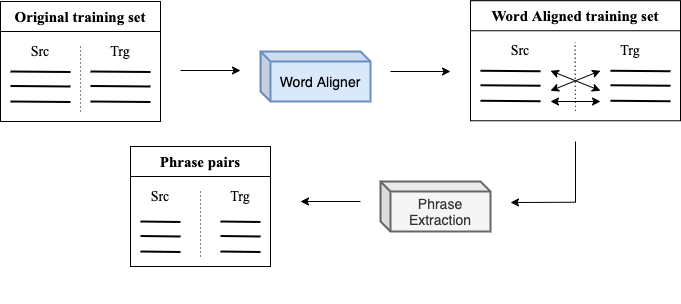
\includegraphics[scale=0.46]{images/phrase_extraction.png}
    \caption{Process of phrase extraction.}
    \label{fig:phrase_extraction}
\end{figure}

\section{Fine-tuning}\label{section:fine-tuning}

%fine-tuning steps : details / phrase datasets
%In Section~\ref{section:pipeline}, we represent the pipeline of our experiments and for both methods, we use fine-tuning. 
%Finetuning refers to continuing to train a pre-trained model on a training set within a domain. 
In Section~\ref{section:pipeline}, we showed the two pipelines of our experiments consisting of the standard and proposed method, respectively. Both methods use fine-tuning, which indicates continuing to train the pre-trained model on an in-domain training set.

To establish an upper bound of the translation quality of domain adaptation, we first conduct the standard method, a common fine-tuning technique for domain adaptation. To do so, we fine-tune the baseline model on full sentences of the original in-domain datasets. 
%For the proposed method, however, the full sentences of the in-domain data are not fed into the NMT system. 
On the other hand, during fine-tuning for the proposed method, we provide phrase pairs to the models as if they were sentence pairs. After the phrase extraction step, the in-domain phrase datasets has many duplicates.
Finally, to study the utility of the phrase pairs, we experiment with various setups for the fine-tuning process. 
%and this will be covered in Section~\ref{section:experiments}

% In this work, we focus on how to effectively use phrases for fine-tuning. %Our main idea is to fine-tune different lengths of phrases to examine the usefulness of them and see if this could benefit more from tagging technique. 
% The main point of our research is to examine the effect of using phrases with different maximum lengths on the fine-tuned models' performance. Furthermore we aim to find out how different phrase lengths interact with our tagging technique.
% %Based on this, we experiment different ways to sub-sample the set of pairs used for fine-tuning.

\subsection{Varying maximum phrase lengths}

To explore the difference in the efficiency of phrases of different length, we fine-tune by using various maximum phrase lengths. Although the sentence structure or context information is all broken, we conjecture the NMT model can learn new terminology from fine-tuning on maximum length 1, equivalent to a dictionary of the in-domain dataset. The longer the phrase (max lengths 4 and 7), the richer the amount of in-domain information for domain adaptation the phrase is expected to hold.

\subsection{Tagging}

As explained in Section~\ref{section:tagging}, we hypothesise that a tagging technique on phrases can prevent the short output bias in phrase-adapted NMT models.
%Phrase pairs differ from the full sentences that the baseline model previously trained on and training NMT models on such short segments can cause a bias that generates shorter output translation. We hypothesise that a tagging technique \parencite{sennrich2016controlling} can prevent this bias in our NMT models. 
We experiment with a simple tagging technique by adding <PT> and </PT> at the front and end of each phrase respectively, in both source and target side. During testing, full sentences with no tags are given to the model. Table~\ref{tab:tagged_phrase_example} shows an example of a source-target pair of full sentences and a pair of phrases with tags from the EMEA dataset. 
%For instance, consider the following German-English phrases pair:\\

\begin{table}[hb!]
\centering
\begin{tabular}{P{0.145\linewidth}| P{0.03\linewidth}| p{0.75\linewidth}}
\Xhline{3\arrayrulewidth}
 & De &
  In den meisten Fällen wird der Serumferritinwert simultan zum Anstieg des \textcolor{blue}{Hämatokritwertes abfallen} . \\ \cline{2-3}
\multirow{-2}{*}{\textbf{Sentence}} &
  En &
  In most cases , the ferritin values in the serum fall simultaneously with the rise in \textcolor{blue}{packed cell volume} .
 \\ \hline\hline
                              & De & {<PT> Hämatokritwertes abfallen </PT>} \\ \cline{2-3}
\multirow{-2}{*}{\textbf{Phrase $+$tags}} & En & <PT> packed cell volume </PT>                             \\ \Xhline{3\arrayrulewidth}
\end{tabular}
\caption{A sample of a pair of full sentences and a phrase pair with tags. The phrases are extracted from the given sentences.}
\label{tab:tagged_phrase_example}
\end{table}

% \begin{table}[hb]
% \centering
% \begin{tabular}{P{0.03\linewidth}| p{0.9\linewidth}}
% \Xhline{3\arrayrulewidth}
% \multicolumn{2}{c}{\textbf{Original sentence}}                                                                      \\ \hline\hline
% \multicolumn{1}{c|}{\textbf{De}} &
%   In den meisten Fällen wird der Serumferritinwert simultan zum Anstieg des \textcolor{blue}{Hämatokritwertes abfallen} \\ 
% \multicolumn{1}{c|}{\textbf{En}} &
%   In most cases , the ferritin values in the serum fall simultaneously with the rise in \textcolor{blue}{packed cell volume} . \\ \hline
% \multicolumn{2}{c}{\textbf{Phrases with tags}}                                                                      \\ \hline\hline
% \multicolumn{1}{c|}{\textbf{De}} & <PT> Hämatokritwertes abfallen </PT> \\ 
% \multicolumn{1}{c|}{\textbf{En}} & <PT> packed cell volume </PT>        \\ \Xhline{3\arrayrulewidth}
% \end{tabular}
% \caption{A sample of a pair of full sentences and a phrase pair with tags. The phrases are extracted from the given sentences.}
% \label{tab:tagged_phrase_example}
% \end{table}

\subsection{Fine-tuning Hyperparameters}

We apply the hyper-parameters described by \cite{ng-etal-2019-facebook} with only a few adjustments inspired from previous work on fine-tuning regularization~\parencite{miceli-barone-etal-2017-regularization}. Specifically, the learning rate is divided by 4 (0.000175) and  for early stopping, we use a small (full-sentence) validation set in each domain (150 sentences, see Table~\ref{tab:data_description}). We set the weight decay rate to 0.0001 and dropout probability to 0.2 after varying experiments. All details of other parameters of the fine-tuning are described in Table~\ref{tab:hyperparameter}.
%only alter the learning rate to 4 times smaller (0.000175). 
%In addition, fine-tuning large NMT models on relatively small in-domain datasets for domain adaptation can be difficult due to a risk of overfitting. 
%To prevent overfitting, we use several techniques: early stopping, drop out \cite{srivastava2014dropout} and weight decay. Especially, \cite{miceli-barone-etal-2017-regularization} reported that early stopping can prevent overfitting, even though it requires held-out training dataset (validation dataset). We fine-tuned several times to discover the optimal setup for each of the full sentences and phrases in each domain. After varying experiments, we set the weight decay rate as 0.0001 and dropout probability as 0.2. 
%We evaluate the quality of NMT models by BLEU score (Section~\ref{section:evaluation_metrics}). To compute this, we use \textsc{SacreBLEU}~\parencite{post-2018-call}.\footnote{\url{ https://github.com/mjpost/sacrebleu}}
We run all the experiments on a node with a \textsc{NVIDIA} V100 GPU in the Peregrine high-performance computing (HPC) cluster of the University of Groningen.\footnote{\url{https://portal.hpc.rug.nl/public/start.html}}


\begin{table}[ht!]
\centering
\begin{tabular}{c|c}
\Xhline{3\arrayrulewidth}
\textbf{Hyperparameter}             & \textbf{Value} \\ \hline
Maximum number of tokens in a batch & 4096 tokens    \\ \hline
Optimizer                           & Adam           \\ \hline
Learning rate                       & 0.00017        \\ \hline
Epoch                               & 20             \\ \hline
Best checkpoint metric              & BLEU           \\ \hline
Beam search size                    & 5              \\ \hline
Drop out                            & 0.2            \\ \hline
Weight decay                        & 0.0001         \\ \hline
Label smoothing                     & 0.1            \\ \Xhline{3\arrayrulewidth}
\end{tabular}
\caption{Hyperparameters for all fine-tuning Transformer based baseline (Section~\ref{section:baseline}) experiments.}
\label{tab:hyperparameter}
\end{table}
\chapter{Results and Analysis}\label{chapter:results}
\section{Baseline}

\begin{table}[h]
\centering
\begin{tabular}{cc}
\Xhline{3\arrayrulewidth}
        &  BLEU  \\\hline
EMEA  &  35.52     \\ 
GNOME  & 27.29       \\
JRC  &   29.03        \\\Xhline{3\arrayrulewidth}

\end{tabular}
\caption{SacreBLEU score for pre-trained German $\rightarrow$ English models}
\label{Tab:NMTresults}
\end{table}

\subsection{Finetuning with original dataset}

\begin{table}[h] 
\centering
\begin{tabular}{ccccccc}
\Xhline{3\arrayrulewidth}
Dataset & Learning rate & Batch size & weight decay  & dropout & Epoch  & BLEU \\\hline
EMEA & 5.0E-04 & 4096 & 0.0001 & 0.2 & &       42.44\\ 
GNOME & 1.00E-03 & 4096 & 0 & 0.2 & &    34.12               \\ 
JRC &5.0E-04 & 4096 & 0.0001 &0  & & 54.38       \\ \Xhline{3\arrayrulewidth}


\end{tabular}
\caption{SacreBLEU for finetuning models with original datasets}
\label{Tab:BLEU}
\end{table}
\chapter{Discussion and Conclusion} \label{chapter:conclusion}
In this chapter, we review and summarise our findings. First, we discuss the experimental results by answering research questions in Section~\ref{section:answer_question}. Afterwards, Section~\ref{section:future_work} suggests possible directions for future work regarding our approach and limitation of this thesis work. Finally, we conclude our work in Section~\ref{chapter:results}. 

%In this chapter we start by making a summary of the contributions of this dissertation. Afterwards, we suggest some of the possible directions for future work regarding the proposed methods.
%This research has not fully gone according to plan. A large portion of work went into obtaining the 6L5K Music Corpus, and determining a representation of this data that can be used as input to various neural networks. Still, we argue that the quality of the dataset and the representation of the data are the main areas for improvement. Furthermore, we only tested two types of neural networks and added a third combination of the two. There are a number of improvements that can be attempted, unfortunately outside the scope of this research.

\section{Answer to Research Questions}\label{section:answer_question}

Based on the results that we obtained by fine-tuning NMT systems on phrases with tagging in various target domains, we can answer the research questions we addressed in Section~\ref{section:research_questions}. We will answer the sub-questions and then the main research question.

\subsection{Answer to sub-research questions}

\noindent \textbf{1. How much does the translation quality of out-of-domain models improve over the baseline models when fine-tuning on in-domain phrase pairs?}

\bigskip

We evaluated the translation quality of the NMT systems by BLEU. For an accurate assessment of the performance of our approach, we established the lower and upper bounds of BLEU gain using the baseline and sentence adapted models, respectively. The baseline's BLEU scores are reached 29 (on JRC) $\sim$ 35.5 (on EMEA) in target domain test sets and fine-tuning on in-domain sentences improved them +9.1 BLEU (on GNOME) $\sim$ +25.7 BLEU (on JRC). By the results of fine-tuning on in-domain phrases, we ascertained that the phrase-adapted models boosted their translation quality over the baseline in all domains. The BLEU gains over the non-adapted baseline vary between +7.0 on EMEA and +1.4 on JRC.

\bigskip

\noindent \textbf{2. Does the use of shorter phrases (i.e. more fragmented data) lower translation quality?}

\bigskip

We hypothesised that shorter phrases would be significantly less useful for fine-tuning, but would better preserve confidentiality.
Therefore, we expected that fine-tuning on longer phrases would result in a higher BLEU score. However, by experimenting with different maximum phrase lengths (1, 4 and 7), we observed that longer phrase datasets do not consistently guarantee a better BLEU score. Increasing the maximum length of phrases from 1 to 4 improved the performance of NMT systems in all domains, however from 4 to 7 worsens it in the GNOME and JRC domains.

%We wanted to understand why maximum length 7 datasets actually drop the BLEU scores. 
We suspected that as one of the reasons for this result, the number of overlapping phrases increases as the maximum length increases when extracting phrases. To investigate the effect of reducing overlapping phrases in maximum length 7 datasets, we experimented with a minimum phrase length (5 words). The experimental results showed various aspects depending on the domain. Fine-tuning on the length 5 $\sim$ 7 phrases in the EMEA domain still results in a higher BLEU than a maximum length 4, but in a trivial decrease of the BLEU than a maximum length 7. In the GNOME domain, setting a minimum length of phrases did not have a positive effect on BLEU. However, in the JRC domain, our approach improved BLEU and eventually had a higher BLEU score than fine-tuning on maximum length 4. To sum up, using shorter phrases does not always reduce translation quality, and the effect is domain dependent.

\bigskip

\noindent \textbf{3. Can the phrase adapted NMT model's translation quality be improved by applying tagging techniques to present phrase pairs to the NMT model?}

\bigskip

When fine-tuning NMT systems on phrases, we concerned with a bias: the model generates shorter translations compared to fine-tuning on original sentences. To alleviate this bias, we used the tagging technique on phrases. In general, adding tags on phrases lifted the BLEU scores. Especially, the positive effect of tagging was notable when fine-tuning on dictionary, +1.6 BLEU on JRC and EMEA $\sim$ +3.8 BLEU on GNOME. Only in the EMEA domain with the maximum length of 7, the BLEU score dropped with tagging technique. 

As an additional experiment, we reduced the total number of phrases in the maximum length 7 datasets by removing phrases shorter than 5 words. Here, on EMEA benefit the model's performance by tagging but interestingly, on other domains deteriorated or stayed. 
%Adding tags on phrases in most cases achieved BLEU gains in fine-tuning NMT models. In particular, short phrases (1 $\sim$ 4 words) benefit more from the addition tags than long ones (longer than 4 words). 

\bigskip

\noindent \textbf{4. When fine-tuning the NMT model on phrase pairs, are there any significant differences between different test domains?}

\bigskip

The experimental results showed that the benefits of domain adaptation on phrases depended on domains. We obtained the biggest improvement on the EMEA domain, but still almost 4 BLEU away from the upper bound. On the GNOME domain, we improved the model performance close to the ceiling. However, the results of the JRC domain presented a significant deviation from our expectations. Despite the biggest benefit from domain adaptation, fine-tuning on phrases in the JRC domain achieved diminutive improvements. We conducted analyses to attain a sufficient explanation for this and discovered that some of target language sentences that consist of copies of the corresponding source and its translation. 
According to \cite{pmlr-v80-ott18a}, the ''copies'' of source sentences can cause a significant effect on the translation quality. To investigate whether this noise affects the model's output, we cleaned the copies from the JRC datasets and fine-tuned again on them. This led to completely different results from the previous JRC data set. The maximum gain of the domain adaptation shrank significantly and fine-tuning on phrases nearly reached the ceiling. 

In addition, we observed that the results of the experiments showed all domains have different patterns. Every domain scored the highest BLEU in a different combination of maximum length and tagging technique. On EMEA increase of the maximum length of the phrase was beneficial but on GNOME and JRC this was not the case. The effect of tagging technique differed across domains, especially in maximum length 7. Applying tagging on maximum length 7 phrases benefits on the GNOME and JRC domains but deteriorates on EMEA. 
%: the effect of phrase length and the tagging technique in BLEU differed across domains.
%On the one hand, we also found that the effect of phrase length and the tagging technique in BLEU differed across domains. Every domain scored the highest BLEU in a different combination of maximum length and tagging technique. The trend of 
%Why are they what they are? What meaning can you wrest from them? Are they in accord with accepted theory? What do they mean with respect to your hypothesis? Do your results uphold your assumptions? How do you treat unexpected or inconsistent results? Can you account for them? Do your results suggest that you need to revise your experiments or repeat them? Do they indicate a revised hypothesis? What are the limitations in your methodology? How do your results fit in with the work of others in the field? What additional work can you suggest?
\bigskip
\subsection{Answer to main research question}

\noindent \textbf{In the scenario where the original data is not shareable due to confidentiality issues and \textit{only shuffled phrase pairs} can be released as a compromise, can this benefit downstream NMT quality in any way?}

\bigskip

In this thesis, we considered the scenario where the translation company \textit{\textbf{A}} wants to improve its NMT system by using the fragmented confidential data of the clients. We proposed phrase pairs as a fragmented format of the parallel corpus. After extracting phrases from the original data, we shuffled and randomly sampled them for preserving confidentiality. Then, we fine-tuned an NMT system on them to assess whether the model can take any advantage of it. Our experimental results support that NMT can benefit from fine-tuning on shuffled phrases instead of full sentences. Still, the improvements by fine-tuning on phrases are lower compared to on full sentences, it is a promising finding in practice because our approach does not need any change in architecture or other fine-tuning algorithms.
\bigskip

% \begin{itemize}
    % \item \parencite[]{gilbertcan} also reported that such a small data( similar amount of sentences) can benefit downstream NMT. For this, they used a commercial NMT system such as Google Translate.
    % Therefore, the highly domain specific data can improve NMT quality, despite of the small amount dataset. 
    % \item Different lengths of phrases : duplicates issues Or it can be noisy anyways. 
    % \item (translate one word segments Transformer) If the model only learns to translate long sentences, it might struggle to translate short ones.: repetition problems (probably n-gram issue?) -> look at the output of traning dictionary : Read \cite{park2020decoding} and think!! 
    % % \item WHY JRC always works strangely? : cite -  Analyzing Uncertainty in Neural Machine Translation \\
    % % "A lesser-known example are target sentences which are entirely in the source language, or which are primarily copies of the corresponding source." : This is exactly the case of JRC that has lots of copies. 
    % \item for the better extraction of phrases, train the alignment model with bigger training set : like adding other in-domain publicly available dataset.\\
    % \item Recent techniques to prevent overfitting during fine-tuning \parencite{kirkpatrick2017overcoming,thompson-etal-2019-overcoming} may overcome this problem in future work.
% \end{itemize}

\section{Limitations and Future Work}\label{section:future_work}
%\textcolor{blue}{ We leave improving and evaluating the preservation of confidentiality by releasing partial sequences for future work.}
% quantify confidentiality : how much we can reconstruct original dataset from the phrases ?
%This work poses numerous insights for a very narrow field: Automatic Language Identification (LID) of vocals in music. The results are limited by relatively low accuracies on unseen data, as well as time constraints. As such, there is a lot of potential for future work in this narrow field of LID to improve over the current findings. 

Based on our findings and limitations of this thesis work, we can contemplate several further research. 

\subsection{Quantifying the preservation of confidentiality}
We proposed an initial solution using confidential data for domain adaptation of NMT models by fragmented parallel corpus, phrase pairs. For using such sensitive data in a fragmented format, two aspects should be satisfied: confidentiality and usefulness. In this thesis work, we mainly focused on the latter to examine whether there can be any benefit to using this type of data. On the other hand, we proposed relatively simple methods for preserving confidentiality but have not measured it. In particular, our threat model is that an adversary may reconstruct the original documents, and this can eventually leak the core information. Therefore, the next step would be to quantify the extent of reconstruction of the original document from the phrases, which so far has only been done in the context of (monolingual) N-grams.\parencite{galle2015reconstructing}.
%If it is possible to adjust the idea of this paper to create Bruijn-graph from the phrase pairs in any way, our method can be evaluated in the confidentiality aspect.

% much more realistic circumstances 
\subsection{Experiments in more realistic circumstances }
In this work, we simulated confidential data by using publicly available datasets. Therefore, future work can assess our approach by experimenting with actual confidential data in a more realistic manner. In addition, even if our work concerned more with the reconstruction of the original text, the actual sensitive data may contain sensitive partial information as well. The de-identification techniques are often applied to protect partial information like in clinical documents~\parencite{meystre2010automatic}. It may combine with our approach to have more reliable protection of confidentiality. It would be intriguing to examine how our method can still exploit fine-tuning on phrases from the de-identified dataset, such as certain key segments are deleted or substituted. 
%Note that we have to choose de-identifying methods to maintain the alignments between source and target sentences. 
Note that de-identification methods have to be applied while maintaining the alignments between source and target sentences.

\subsection{Experiments in different setups}
%different setups : model / different languages
Our approach was only tested with a Transformer based model, which has a state-of-art performance in NMT and in German-English, which is known as a high-resource and close language pair. To investigate our method in different setups, we would like to assess the same experiments with different NMT models, such as CNN or LSTM based models, and with other language pairs including low-resource and difficult ones. We also found that the improvements of translation quality of phrase-adapted models are varied across different domains. To explore the difference in more domains, we can experiment with other domains that we did not choose in this paper. 

% New idea - using N-grams 
\subsection{Monolingual fragmented data: N-grams}
Our results show that a fragmented dataset still contains valuable information for fine-tuning an NMT system. We used phrase pairs as fragmented text because they can maintain the alignments of the parallel corpus. However, for some language pairs, the available parallel datasets are limited. As a solution for this, many studies utilising monolingual data for NMT systems have been conducted, and they have shown good results. Therefore, extending our approach, we may consider N-grams as a monolingual dataset. For instance, with 'Back-Translation'\parencite{sennrich-etal-2016-improving} we generate a new pseudo parallel dataset and conduct fine-tuning on them. With this, we may easily apply the methods from ~\cite{galle2015reconstructing}. 


%\cite{galle2015reconstructing} proposed an approach of generating the noised N-grams for preventing reconstruction of the whole original documents. This technique is inspired by de Bruijn graph commonly used in DNA sequence mapping, and noise is added to N-grams. Based on this, future work can adjust the noising technique system and add noise to given phrases. %The noised N-grams will lose utility compared with N-grams thus the proper amount of noise should be investigated.
%conduct a comprehensive study of the privacy implications of our technique similar to \cite{galle2015reconstructing}. 


\section{Conclusion}\label{section:conclusion}
% We believe that our findings have several implications for machine translation research. Most importantly, if we accept our interpretation

% Our in-depth analysis on our method of transferring pretrained models, showed that: 1)

We have studied the problem of domain adaptation of NMT models when domain-specific data cannot be shared due to confidentiality or copyright concerns. Inspired by a common NLP practice of sharing confidential data in the form of N-grams \parencite[]{michel2011quantitative}, we propose to use phrase extraction \parencite{koehn2003statistical}, shuffling and sub-sampling as a data fragmentation technique for translation data.

Our experiments on three different domains show that this type of data can be used to fine-tune NMT models leading to considerable improvements on top of a strong baseline and further gains when using a simple phrase tagging technique. We also find that the magnitude of these gains varies largely across domains. Our analysis and additional experiments show that: 1) fine-tuning on short segments can improve translation of short sentences as well as long sentences 2) it still needs more explanation of what causes the profits difference across domains.

%and offer an initial explanation based on the average length of sentence.
%Reconstructing the full documents from the N-grams is quite challenging\cite{galle2015reconstructing}, therefore fragmented data can be an option for keeping the confidentiality of original documents.

% Bibliography

\printbibliography


% Appendixes
\appendix
% \section{Useful literature}
% This is a place to keep all useful papers and references.
% 
% \begin{itemize}
%     \item General RL
%     \begin{itemize}
%         \item Hindsight Experience Replay \parencite{andrychowicz2017hindsight}
%         \item Prioritized experience replay \parencite{schaul2015prioritized}
%         \item Curiosity-driven exploration \parencite{schmidhuber2010formal}
%     \end{itemize}
%     \item Curriculum learning
%     \begin{itemize}
%         \item Automatic Curriculum Learning For Deep RL: A Short Survey \parencite{portelas2020automatic}
%     \end{itemize}
%     \item HRL
%     \begin{itemize}
%         \item Article that reviews different HRL (\href{https://thegradient.pub/the-promise-of-hierarchical-reinforcement-learning/}{link})
%         \item Overview of HRL \parencite{HRL2011Overview}
%         \item Overview of HRL \parencite{Barto2003}
%         \item HRL Lifelong Learning Minecraft \parencite{tessler2016deep}
%         \item Options framework \parencite{sutton1999options}
%         \item MAXQ \parencite{dietterich2000hierarchical}
%         \item DHRL marco student \parencite{niel2018hierarchical}
%         \item HEXQ automatic hierarchichal strtucture \parencite{hengst2002discovering}
%         \item HABS (Hierarchical Assignment of Behaviours to Subpolicies) \parencite{moermanhierarchical}
%         \item FeUdal Networks (FUN) \parencite{Vezhnevets:2017:FNH:3305890.3306047}
%         \item HIRO Google \parencite{nachum2018HIRO}
%         \item HAC \parencite{levy2018hierarchical}
%         \item MLSH openAI \parencite{frans2017MLSH}
%         \item COBRA: Curiosity \parencite{watters2019cobra}
%         \item Deepmind Object-oriented state editing for HRL \parencite{bapst2019objectoriented}
%     \end{itemize}
%     \item Lifelong Learning
%     \begin{itemize}
%         \item Lifelong Machine Learning \parencite{silver2013lifelong}
%     \end{itemize}
% \end{itemize}



\newcommand{\SH}[1]{{\small\textcolor{blue}{[NOTE: #1]}}}
\end{document}
